\documentclass[a4paper, 11pt]{article}

\usepackage[utf8]{inputenc}
\usepackage{babel}
\usepackage{hyperref}
\usepackage[capitalise, noabbrev]{cleveref}
\usepackage{a4wide}
\usepackage{relsize}
\usepackage{indentfirst}
\usepackage{nameref}
\usepackage{graphicx}
\usepackage{float}
\usepackage[cache=false]{minted}
\usepackage[normalem]{ulem}
\usepackage{setspace}
\usepackage{color}

\onehalfspacing

\hypersetup{
    pdftitle={Advanced Topics in Databases},
    pdfborder={0 0 0}
}

\title{Advanced Topics in Databases \\ [0.8em] \smaller Practical Assignment}
\author{Aníbal Silva \and Rui Fernandes}
\date{\today}

\begin{document}

\renewcommand\labelitemi{--}
\renewcommand{\today}{\ifcase \month\or January\or February\or March\or %
April\or May\or June\or July\or August\or September\or October\or November\or %
December\fi, \number \year}

\begin{titlepage}
    \begin{center}
        \begin{minipage}{.75\linewidth}
            \centering
            
\includegraphics[width=0.5\textwidth]{img/fcup}\par\vspace{1cm}
            \vspace{1.5cm}
            {\scshape\LARGE Faculty of Sciences of the University of Porto} \par
            \vspace{1cm}
            {\scshape\Large Department of Computer Science} \par
            \vspace{1.5cm}
            \maketitle
        \end{minipage}
    \end{center}
    \vspace{2cm}
    \thispagestyle{empty}
    \pagebreak
\end{titlepage}

\pagebreak

\pagenumbering{roman}

\begin{abstract}
This report describes the practical assignment of the Advanced Topics in Databases course. 

This practical assignment consists in creating a data warehouse and conducting data analysis on it, as well as creating
graphical reports using the Python library \texttt{matplotlib}.

In this report, we briefly describe our approach to the problem and discuss the decisions we made.
\end{abstract}

\pagebreak

\tableofcontents \pagebreak
\listoffigures \pagebreak

\pagenumbering{arabic}

\section{Introduction}

The data warehouse contains data from national swimming competitions at the master level (\textit{i.e.} class of
competitive swimming for swimmers 25 years and older), namely Troféu Pescada 2021 and the Summer 2021 Championship.

\textcolor{red}{COMPLETAR COM TEXTO}

\subsection*{Structure of the Report}

The remainder of the report is structured as follows:

\begin{itemize}
    \item In \cref{sec:data-model}, \textbf{\nameref{sec:data-model}}, we describe the data contained in the data warehouse.
    \item In \cref{sec:analysis}, \textbf{\nameref{sec:analysis}}, we provide some insight into the data by looking into relevant
    statistics as well as plotting the data we considered relevant.
    \item Finally, \cref{sec:conclusion}, \textbf{\nameref{sec:conclusion}}, concludes the report and suggests remarks
    for future work.
\end{itemize}

\pagebreak

\section{Data Model} \label{sec:data-model}

\vspace{\baselineskip}

In this section, we describe the data tables contained in the data warehouse. 

Some modifications were made in the original script. This was mainly motivated due to the fact that same athletes and clubs had different
\texttt{ids} for different meets, when in our perspective they should be uniquely identified across tournaments. They were defined as: 

\vspace{\baselineskip}

\begin{itemize}
    \item \texttt{athleteid} = \texttt{firstname} + \texttt{lastname} + \texttt{birthdate} + \texttt{inc\_id}, where the \texttt{inc\_id} increments when two athletes share the same first and last name and the birthdate;
    \item \texttt{clubid} = \texttt{code} + \texttt{nation} + \texttt{region};
    \item \texttt{resultid} = \texttt{meetid} + \texttt{resultid};
    \item \texttt{swimstyleid} = \texttt{distance} + \texttt{relaycount} + \texttt{stroke};
    \item \texttt{eventid} = \texttt{meetid} + \texttt{eventid};
    \item The \texttt{license}, which originally was \texttt{meetid} + \texttt{clubid} + \texttt{idx} was replaced by \texttt{athleteid} + \texttt{meetid} because the same athlete could have changed between teams for different tournaments.
\end{itemize}

\vspace{\baselineskip}

Regarding our data model, we built two fact tables, one that gathers information regarding a club in a tournament, while another gathered 
information of a given athlete in a tournament. Our schema is illustrated in \cref{fig:defact}. 

\begin{figure}[H]
    \centering
    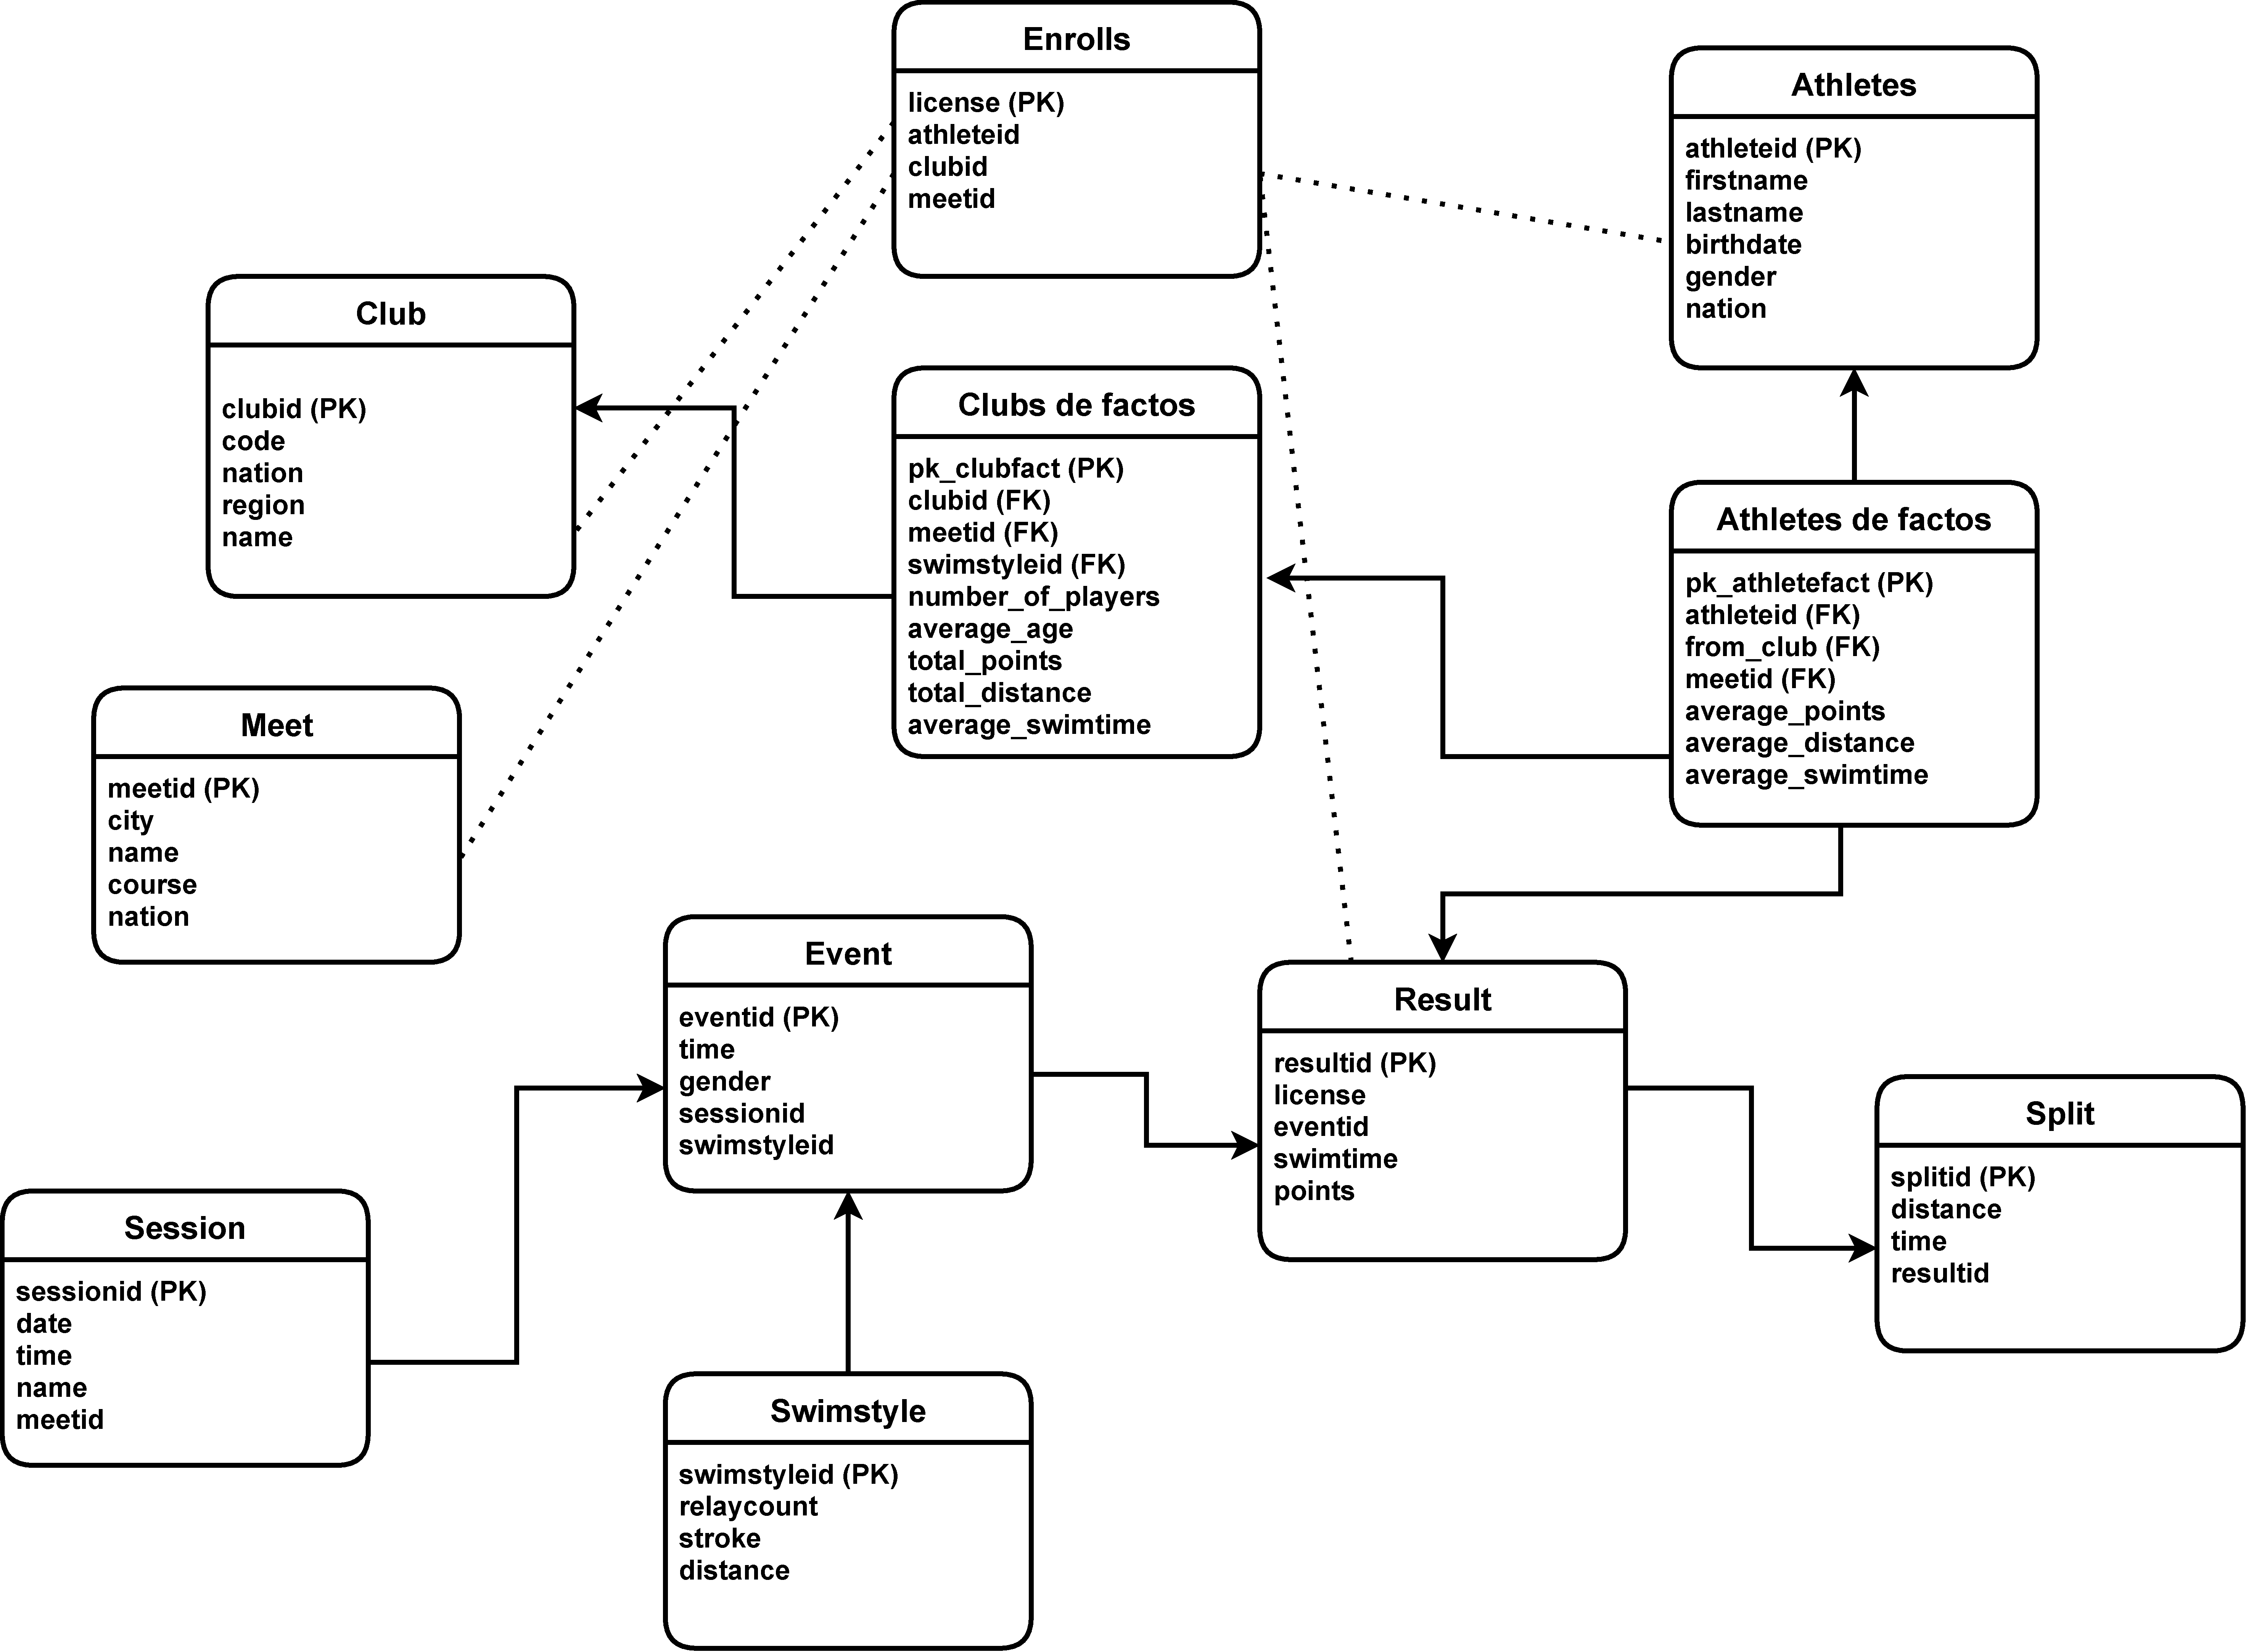
\includegraphics[width=\textwidth]{img/datawarehouse.pdf}
    \caption{Datawarehouse schema}
    \label{fig:defact}
\end{figure}

This Figure shows two fact tables, one related to overall statistics of a team in a tournament, while the other containing the overall statistics of an athlete. Regarding the first table, \textit{Club de factos}, we grouped our data by \texttt{meetid}, \texttt{clubid} and \texttt{swimstyleid} to extract the following statistics:

\begin{itemize}
    \item \texttt{number\_of\_players} - the number of players;
    \item \texttt{average\_age} - the average age of players;
    \item \texttt{total\_points} - the total points a given team had in a tournament;
    \item \texttt{total\_distance} - the total distance all the players swam in a team;
    \item \texttt{average\_swimtime} - the average swimtime all the players swam.
\end{itemize}

Regarding the second fact table, \textit{Athletes de factos}, we grouped our data by \texttt{athleteid}, \texttt{meetid} and \texttt{from\_club} in order to extract the following statistics:

\begin{itemize}
    \item \texttt{average\_swimtime} - The average swimtime a given athlete swam
    \item \texttt{average\_points} - The average points an athlete had
    \item \texttt{average\_distance} - The average distance an athlete swam
\end{itemize}

for a given tournament.

\pagebreak

\section{Data Analysis \& Visualization} \label{sec:analysis}

In this section, we \textcolor{red}{completar com texto}.

\subsection{Athletes by Age}

To determine to determine the average age of the athletes, we can run the following SQL query:

\begin{minted}{sql}
SELECT AVG(age(birthdate))
FROM annp_final.athlete;
\end{minted}

From this, we can see that the average age of the athletes is 46 years, 6 months and 31 days.

We can also determine who's the youngest athlete by running the following SQL query:

\begin{minted}{sql}
SELECT *
FROM annp_final.athlete
ORDER BY age(birthdate) ASC
LIMIT 1;
\end{minted}

\begin{itemize}
    \item \textbf{Name:} Ana Mónica Eloi
    \item \textbf{Gender:} Female
    \item \textbf{Birthdate:} 29/12/1996
    \item \textbf{Age:} 25 years
\end{itemize}

On the other hand, we can learn information about the oldest athlete by running the following SQL query:

\begin{minted}{sql}
SELECT *
FROM annp_final.athlete
ORDER BY age(birthdate) DESC
LIMIT 1;
\end{minted}

\begin{itemize}
    \item \textbf{Name:} Virgílio Zacarias Costa
    \item \textbf{Gender:} Male
    \item \textbf{Birthdate:} 21/07/1931
    \item \textbf{Age:} 90 years
\end{itemize}

Finally, to determine the number of athletes by age, we can run the following SQL query using the PostgreSQL's built-in
\texttt{age} function:

\begin{minted}{sql}
SELECT
    COUNT(*),
    EXTRACT(YEAR FROM age(birthdate)) AS age
FROM annp_final.athlete
GROUP BY age
ORDER BY age ASC;
\end{minted}

We can then plot the result, as illustrated in \cref{fig:athletesbyage}.

\vspace{\baselineskip}

\begin{figure}[H]
    \centering
    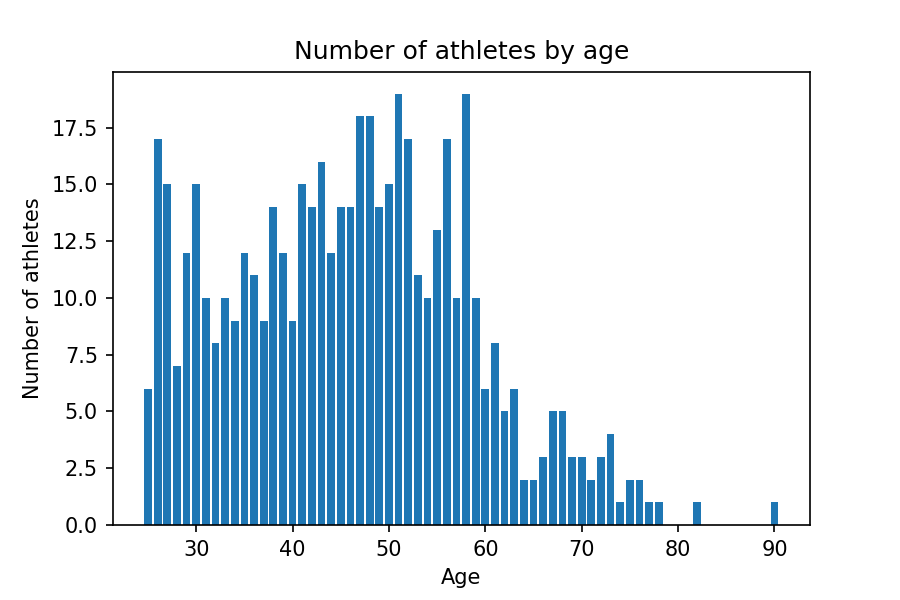
\includegraphics[width=.8\textwidth]{img/athletesbyage.png}
    \caption{Number of athletes by age}
    \label{fig:athletesbyage}
\end{figure}

We can also plot the number of athletes by age based on their gender, as illustrated in \cref{fig:athletesbyageandgender}.
To do so, we have to run the following SQL query:

\begin{minted}{sql}
SELECT 
    EXTRACT(YEAR FROM age(birthdate)) AS age,
    gender,
    COUNT(*)
FROM annp_final.athlete
GROUP BY (age, gender)
ORDER BY age ASC;
\end{minted}

\begin{figure}[H]
    \centering
    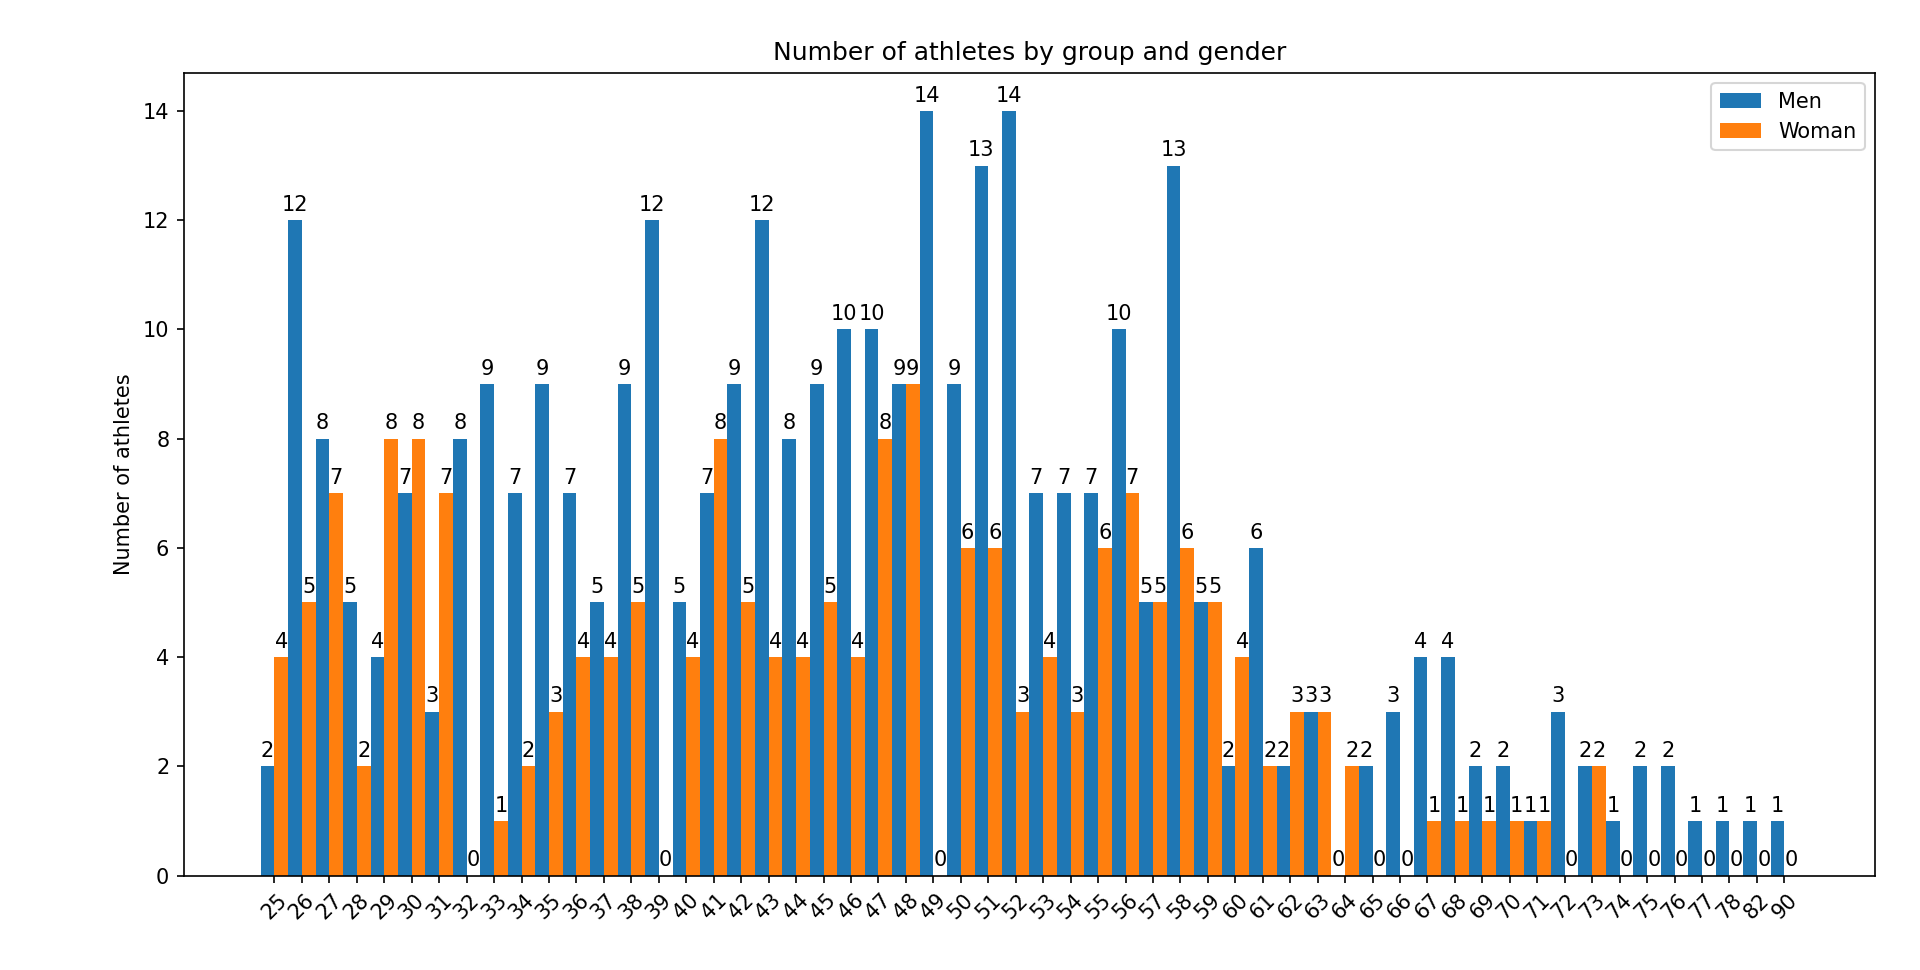
\includegraphics[width=\textwidth]{img/athletesbyageandgender.png}
    \caption{Number of athletes by age and gender}
    \label{fig:athletesbyageandgender}
\end{figure}

\subsection{Athletes by Nation}

To determine the number of athletes by nation, we can run the following SQL query:

\begin{minted}{sql}
SELECT
    nation,
    COUNT(*) AS nationCount
FROM annp_final.athlete
GROUP BY nation
ORDER BY nationCount ASC;
\end{minted}

We can then plot the result, as illustrated in \cref{fig:athletesbynation}.

\begin{figure}[H]
    \centering
    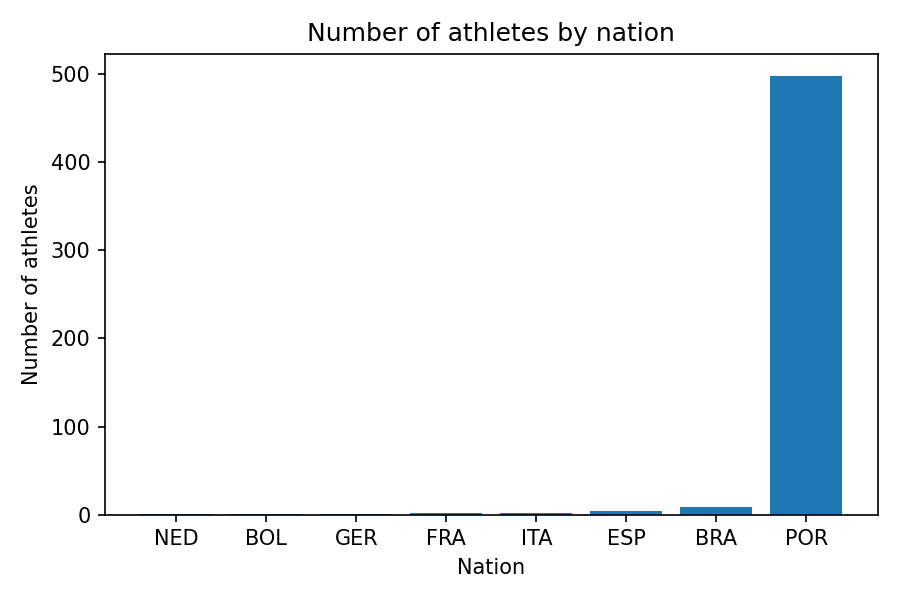
\includegraphics[width=.65\textwidth]{img/athletesbynation.png}
    \caption{Number of athletes by nation}
    \label{fig:athletesbynation}
\end{figure}

We can also take the gender into account with following SQL query:

\begin{minted}{sql}
SELECT 
    nation,
    gender,
    COUNT(*)
FROM annp_final.athlete
GROUP BY CUBE (nation, gender)
ORDER BY nation, gender NULLS LAST;
\end{minted}

Plotting the result, we have the following:

\begin{figure}[H]
    \centering
    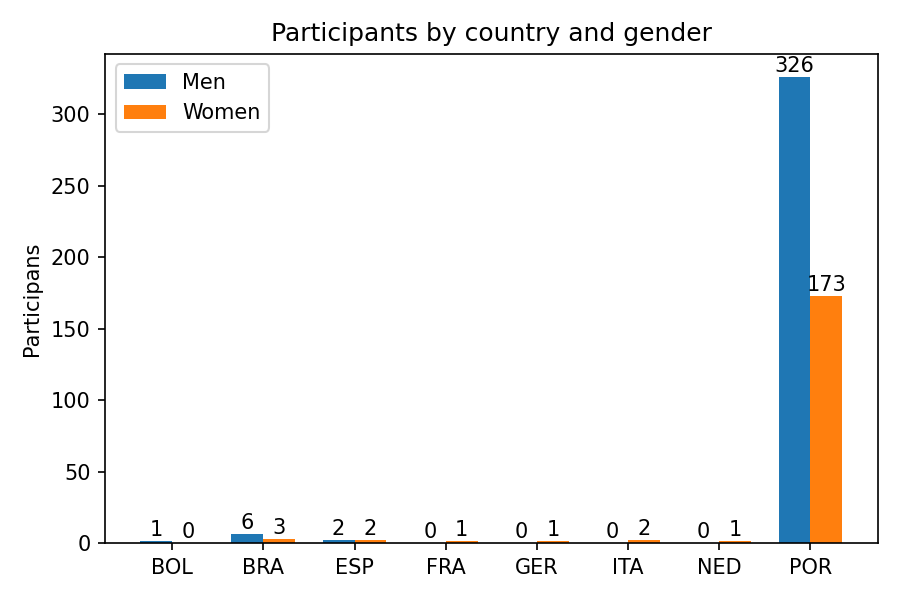
\includegraphics[width=.65\textwidth]{img/athletesbynationgender.png}
    \caption{Number of athletes by nation and gender}
    \label{fig:athletesbynationgender}
\end{figure}

\subsection{Athletes by Gender}

To determine the number of athletes by gender, we can run the following SQL query:

\begin{minted}{sql}
SELECT
    gender,
    COUNT(*)
FROM annp_final.athlete
GROUP BY gender;
\end{minted}

We can then plot the result, as illustrated in \cref{fig:athletesbygender}.

\begin{figure}[H]
    \centering
    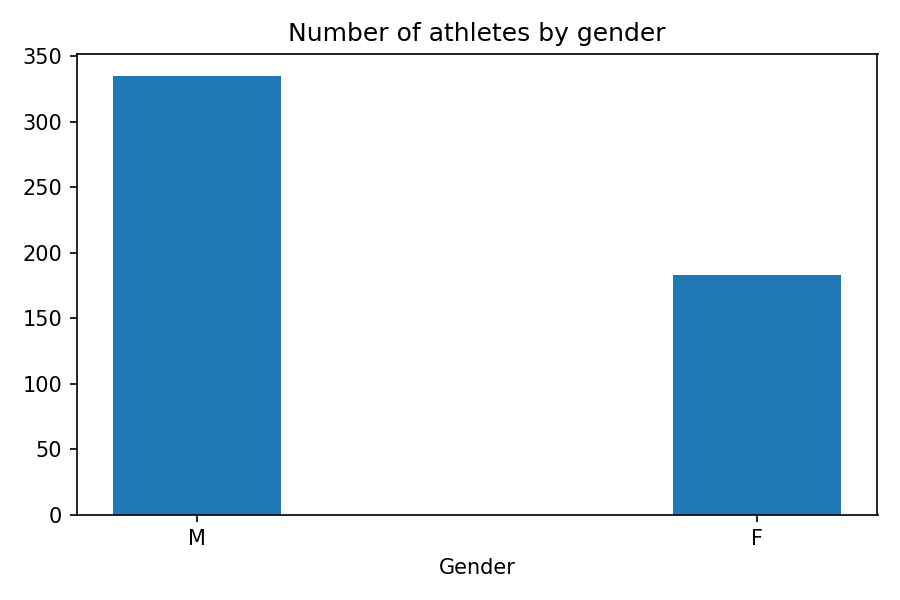
\includegraphics[width=.65\textwidth]{img/athletesbygender}
    \caption{Number of athletes by gender}
    \label{fig:athletesbygender}
\end{figure}

We can also plot this in a pie chart, as illustrated in \cref{fig:athletesbygender-pie}.

\begin{figure}[H]
    \centering
    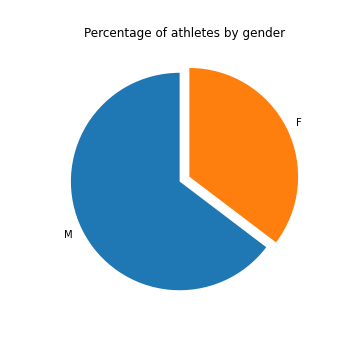
\includegraphics[width=.65\textwidth]{img/athletesbygender-pie}
    \caption{Percentage of athletes by gender}
    \label{fig:athletesbygender-pie}
\end{figure}

\subsection{Events by Gender}

To determine the number of events by gender, we can run the following SQL query:

\begin{minted}{sql}
SELECT
    gender,
    COUNT(*)
FROM annp_final.event
GROUP BY gender;
\end{minted}

We can then plot the result, as illustrated in \cref{fig:eventsbygender}.

\begin{figure}[H]
    \centering
    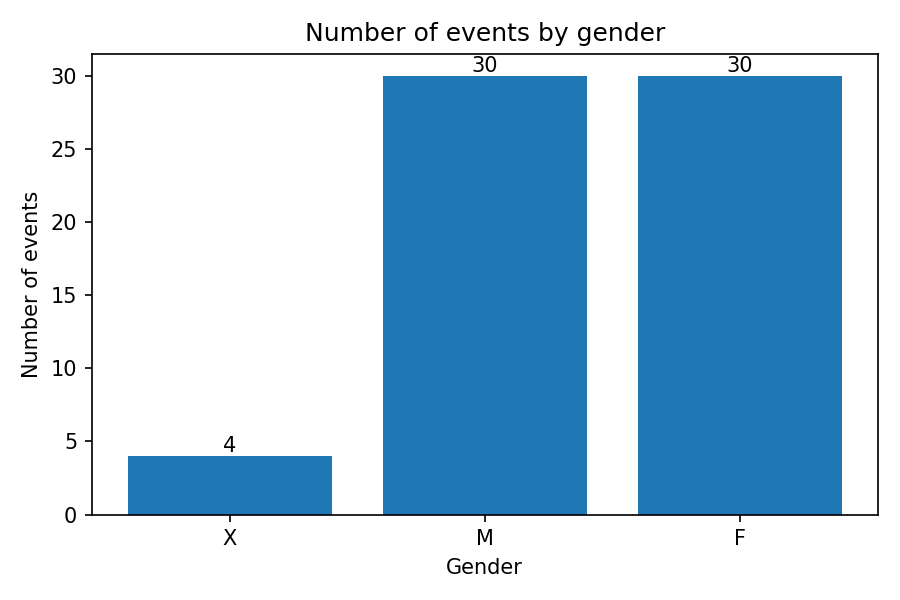
\includegraphics[width=.6\textwidth]{img/eventsbygender}
    \caption{Number of events by gender}
    \label{fig:eventsbygender}
\end{figure}

Here, the value \texttt{X} refers to events that allow athletes from both genders to participate.
We can also plot this in a pie chart, as illustrated in \cref{fig:eventsbygender-pie}.

\begin{figure}[H]
    \centering
    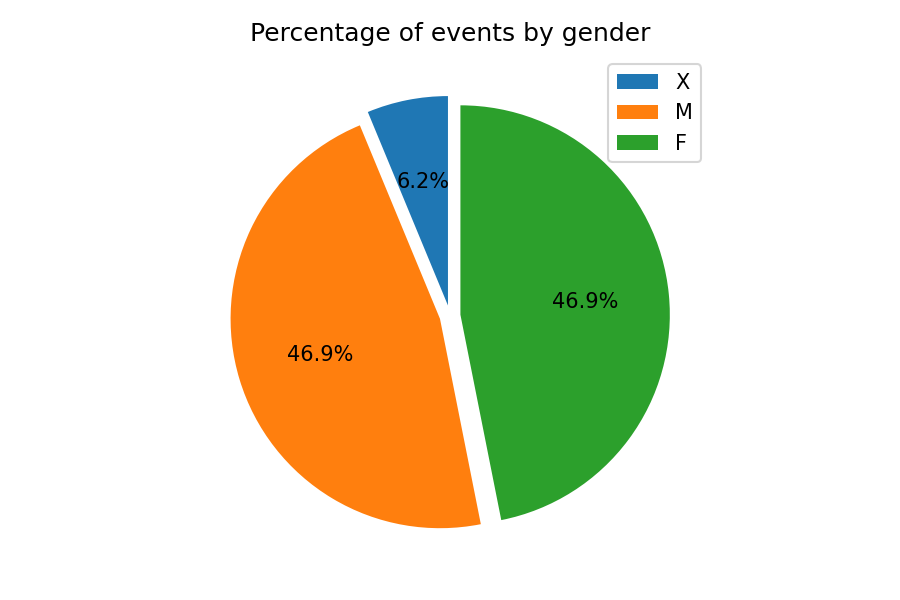
\includegraphics[width=.65\textwidth]{img/eventsbygender-pie}
    \caption{Percentage of events by gender}
    \label{fig:eventsbygender-pie}
\end{figure}

\subsection{Number of Clubs by Nation}

We can determine the number of clubs by each nation by running the following SQL query:

\begin{minted}{sql}
SELECT
    nation,
    COUNT(*) AS nationCount
FROM annp_final.club
GROUP BY nation
ORDER BY nationCount ASC;
\end{minted}

Plotting the result in a bar chart, we have the following:

\begin{figure}[H]
    \centering
    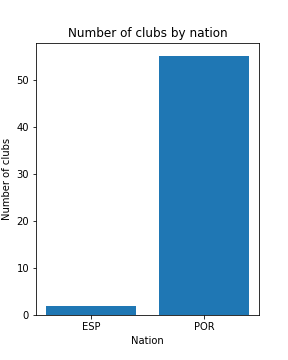
\includegraphics[width=.6\textwidth]{img/clubsbynation}
    \caption{Number of clubs by nation}
    \label{fig:clubs-by-nation}
\end{figure}

We can also plot this in a pie chart, which gives us the following:

\begin{figure}[H]
    \centering
    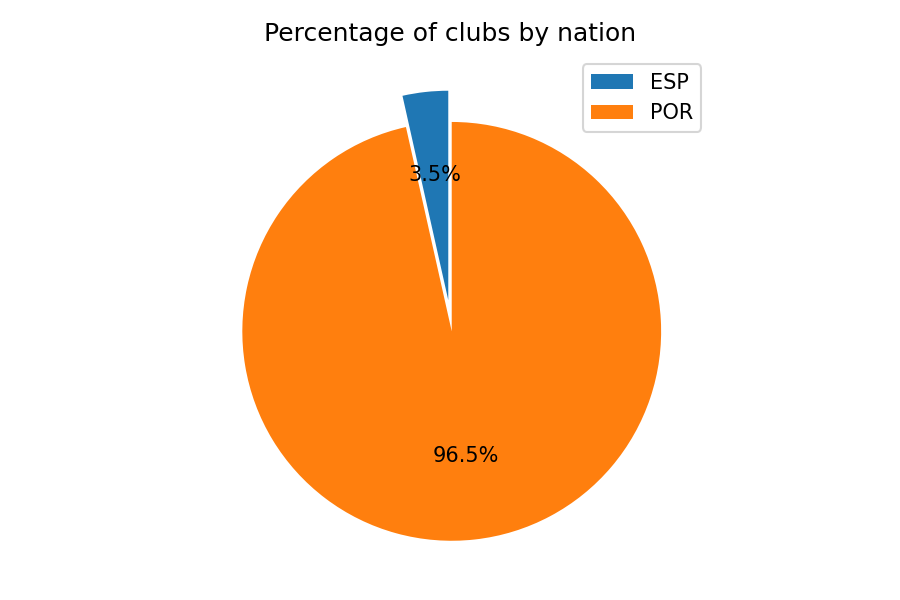
\includegraphics[width=.65\textwidth]{img/clubsbynation-pie}
    \caption{Percentage of clubs by nation}
    \label{fig:clubs-by-nation-pie}
\end{figure}

\subsection{Clubs by Region}

To determine the number of clubs per each region in Portugal, we can run the following SQL query:

\begin{minted}{sql}
SELECT 
    region,
    COUNT(*) AS regionCount
FROM annp_final.club
WHERE region SIMILAR TO '[A-Z]+'
GROUP BY region
ORDER BY regionCount ASC;
\end{minted}

Plotting the result of the query in a bar chart we have the following:

\vspace{.5\baselineskip}

\begin{figure}[H]
    \centering
    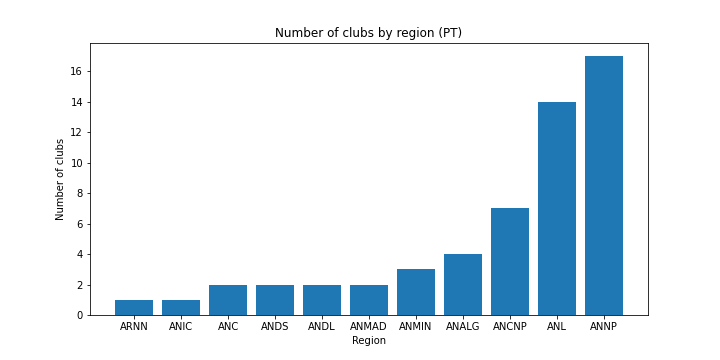
\includegraphics[width=.85\textwidth]{img/clubsbyregion-pt.png}
    \caption{Number of clubs by region}
    \label{fig:clubs-by-region-pt}
\end{figure}

\vspace{.5\baselineskip}

Here, it is worth noting that this query only considers the portuguese clubs, because each is identified by uppercase
letters only.
Spanish regions, on the other hand, are identified with numbers, which means that if we want to run the previous query
considering only spanish regions, we only have to replace \texttt{WHERE region SIMILAR TO '[A-Z]+'} with
\texttt{WHERE region SIMILAR TO '[0-9]+'}, as shown bellow:

\pagebreak

\begin{minted}{sql}
SELECT
    region,
    COUNT(*) AS regionCount
FROM annp_final.club
WHERE region SIMILAR TO '[0-9]+'
GROUP BY region
ORDER BY regionCount ASC;
\end{minted}

However, this has a downside in the sense that we have no way of knowing which regions these values \texttt{10114} and
\texttt{11115} refer to.
Ploting the result in a bar plot, we have the following:

\begin{figure}[H]
    \centering
    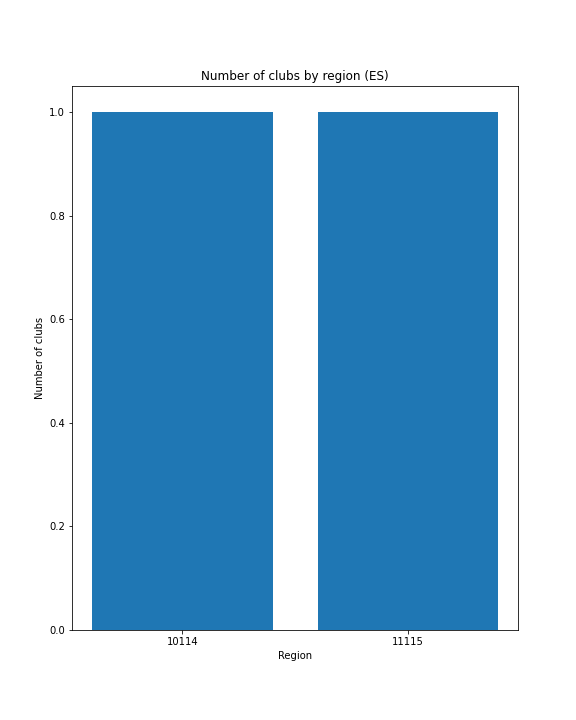
\includegraphics[width=.6\textwidth]{img/clubsbyregion-es}
    \caption{Number of clubs by region (ES)}
    \label{fig:clubs-by-region-es}
\end{figure}

We can also plot this a pie chart, which gives us the following:

\begin{figure}[H]
    \centering
    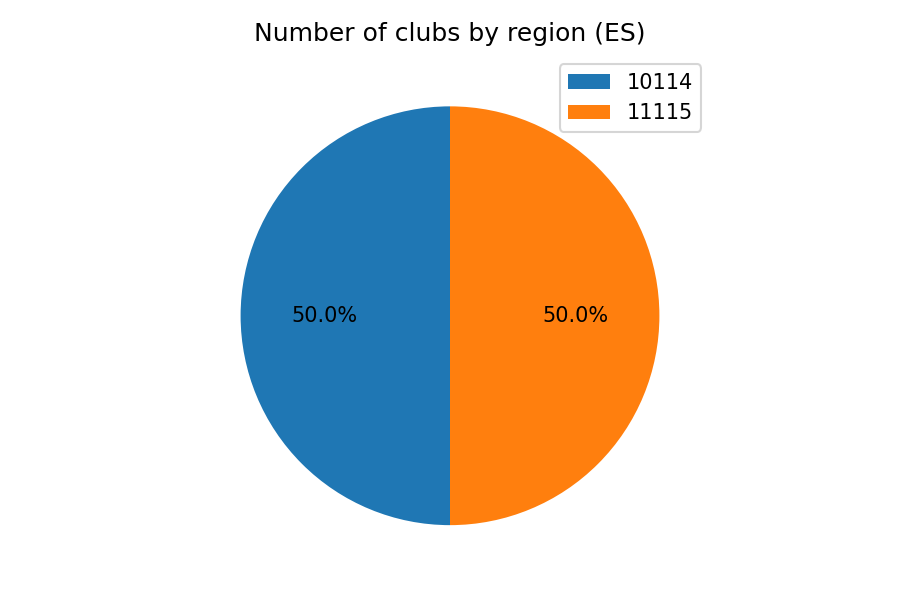
\includegraphics[width=.6\textwidth]{img/clubsbyregion-es-pie}
    \caption{Number of clubs by region (ES)}
    \label{fig:clubs-by-region-es-pie}
\end{figure}

\subsection{Club facts statistics}

\subsubsection{Overall Statistics}

Given the Club facts table, we can plot some of their statistics. Below, we present a query that fetches these statistics for all possible combinations
between \texttt{meetid} and \texttt{clubid}. Note that instead we used the \texttt{code} column from \texttt{club} table to easily read each team for 
a given tournament. 

\begin{minted}{sql}
SELECT 
CASE GROUPING(cd.meetid)
    WHEN 1 THEN 'all_meets'
    ELSE cd.meetid
END AS "Tournament",
CASE GROUPING(c.code)
    WHEN 1 THEN 'all_clubs'
    ELSE c.code
END AS "Team",
   ROUND(AVG(average_age), 0) AS "Average Age",
   ROUND(AVG(average_swimtime), 2) AS "Average Swimtime",
   ROUND(SUM(total_points)) AS "Total Points",
   ROUND(SUM(number_of_players)) AS "Total Players"
FROM (
    SELECT CAST(meetid AS VARCHAR(255)),
       clubid,
       average_age,
       total_points,
       average_swimtime,
       number_of_players
    FROM annp_final.club_defacto) cd
JOIN annp_final.club c ON c.clubid = cd.clubid
GROUP BY CUBE (cd.meetid, c.code);
\end{minted}

\begin{figure}[H]
    \centering
    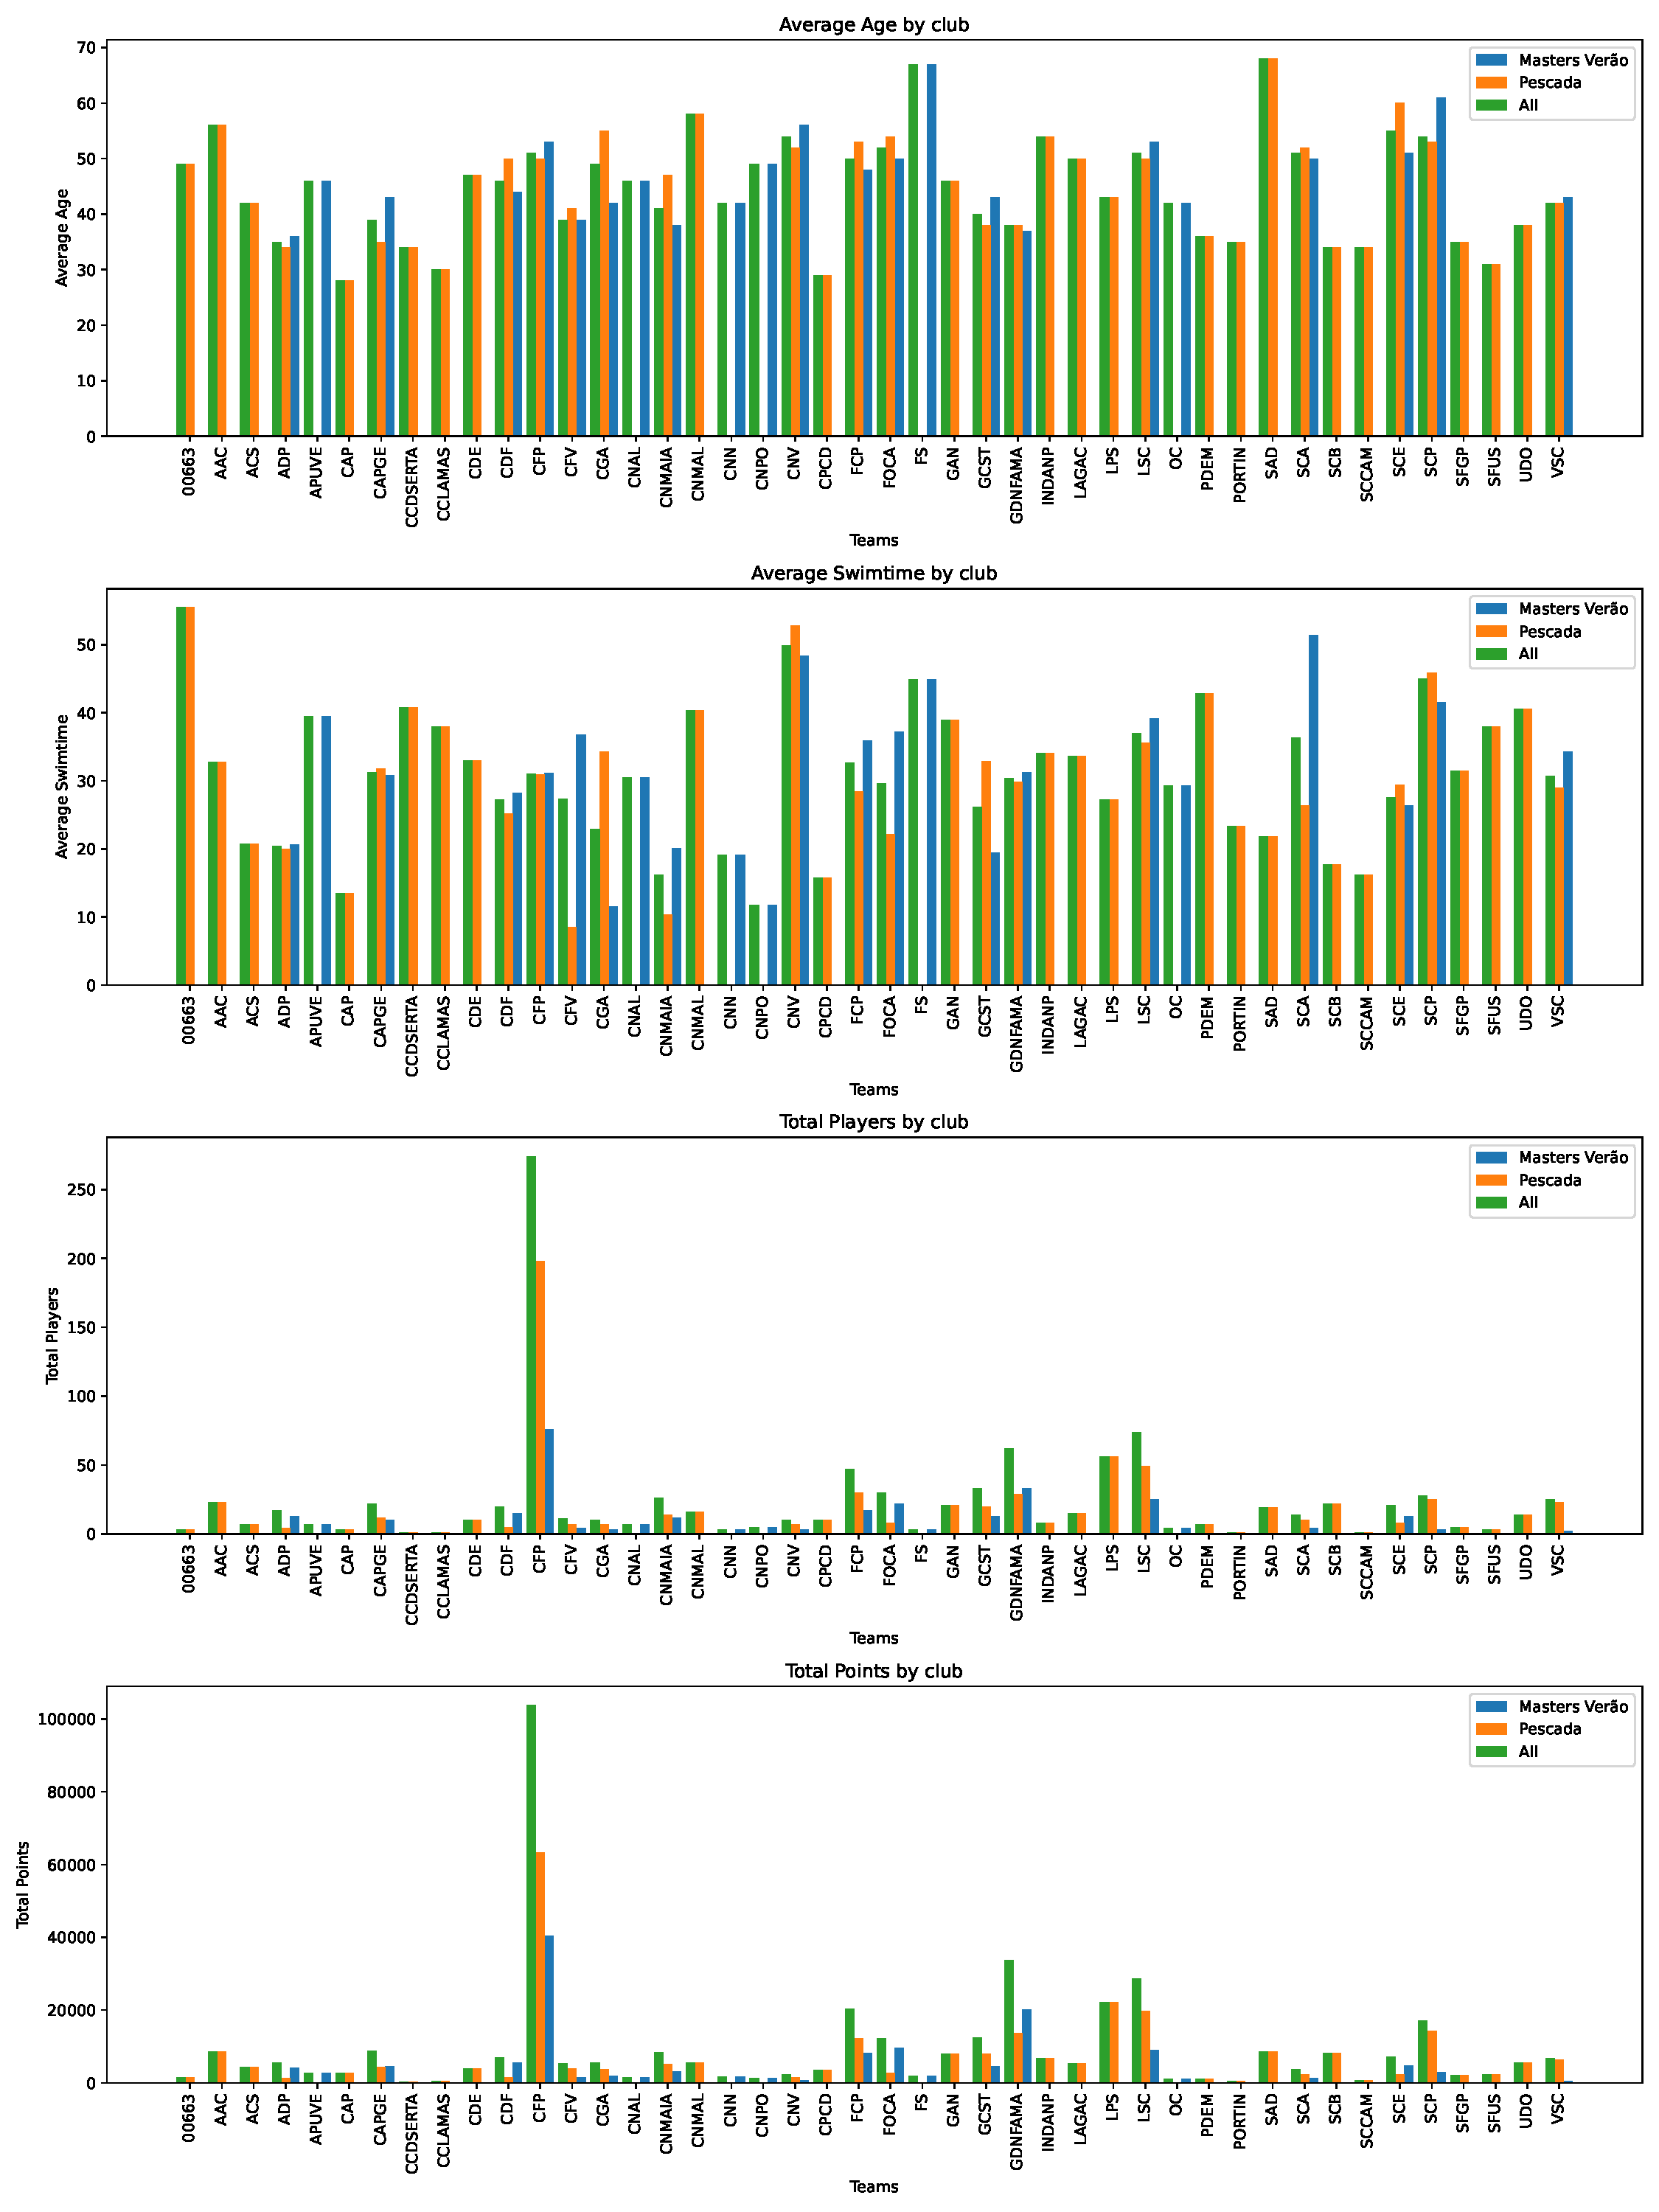
\includegraphics[width=\textwidth]{img/club_fact1.pdf}
    \caption{Statistics from fact Club table.}
    \label{fig:clubs_fact}
\end{figure}

\subsubsection{Statistics for a given Swim Style}

Next, we also show the overall statistics given a swim style. For that, we use the following SQL query:

\begin{minted}{sql}
SELECT 
    CASE GROUPING(c.code)
        WHEN 1 THEN 'all_clubs'
        ELSE c.code
    END AS "Team",
    CASE GROUPING(cd.swimstyleid)
        WHEN 1 THEN 'all_styles'
        ELSE cd.swimstyleid
    END AS "SwimStyle",
    ROUND(AVG(average_swimtime), 2) AS "Average Swimtime",
    ROUND(SUM(total_points)) AS "Total Points",
    ROUND(SUM(number_of_players)) AS "Total Players"
FROM annp_final.club_defacto cd
JOIN annp_final.club c on c.clubid = cd.clubid
GROUP BY CUBE (c.code, cd.swimstyleid)
ORDER BY "Total Points" DESC
\end{minted}

To filter the amount of information this table has, we filter, for a given swim style, the top 5 teams that had the higher total of points. This is done for all the
tournaments. This pre-processing step was done in Python and the result is depicted in \cref{fig:clubs_fact2}. Note that not all the bar plots have 5 teams. This
is due to the lack of data presented from both tournaments.

\begin{figure}[H]
    \centering
    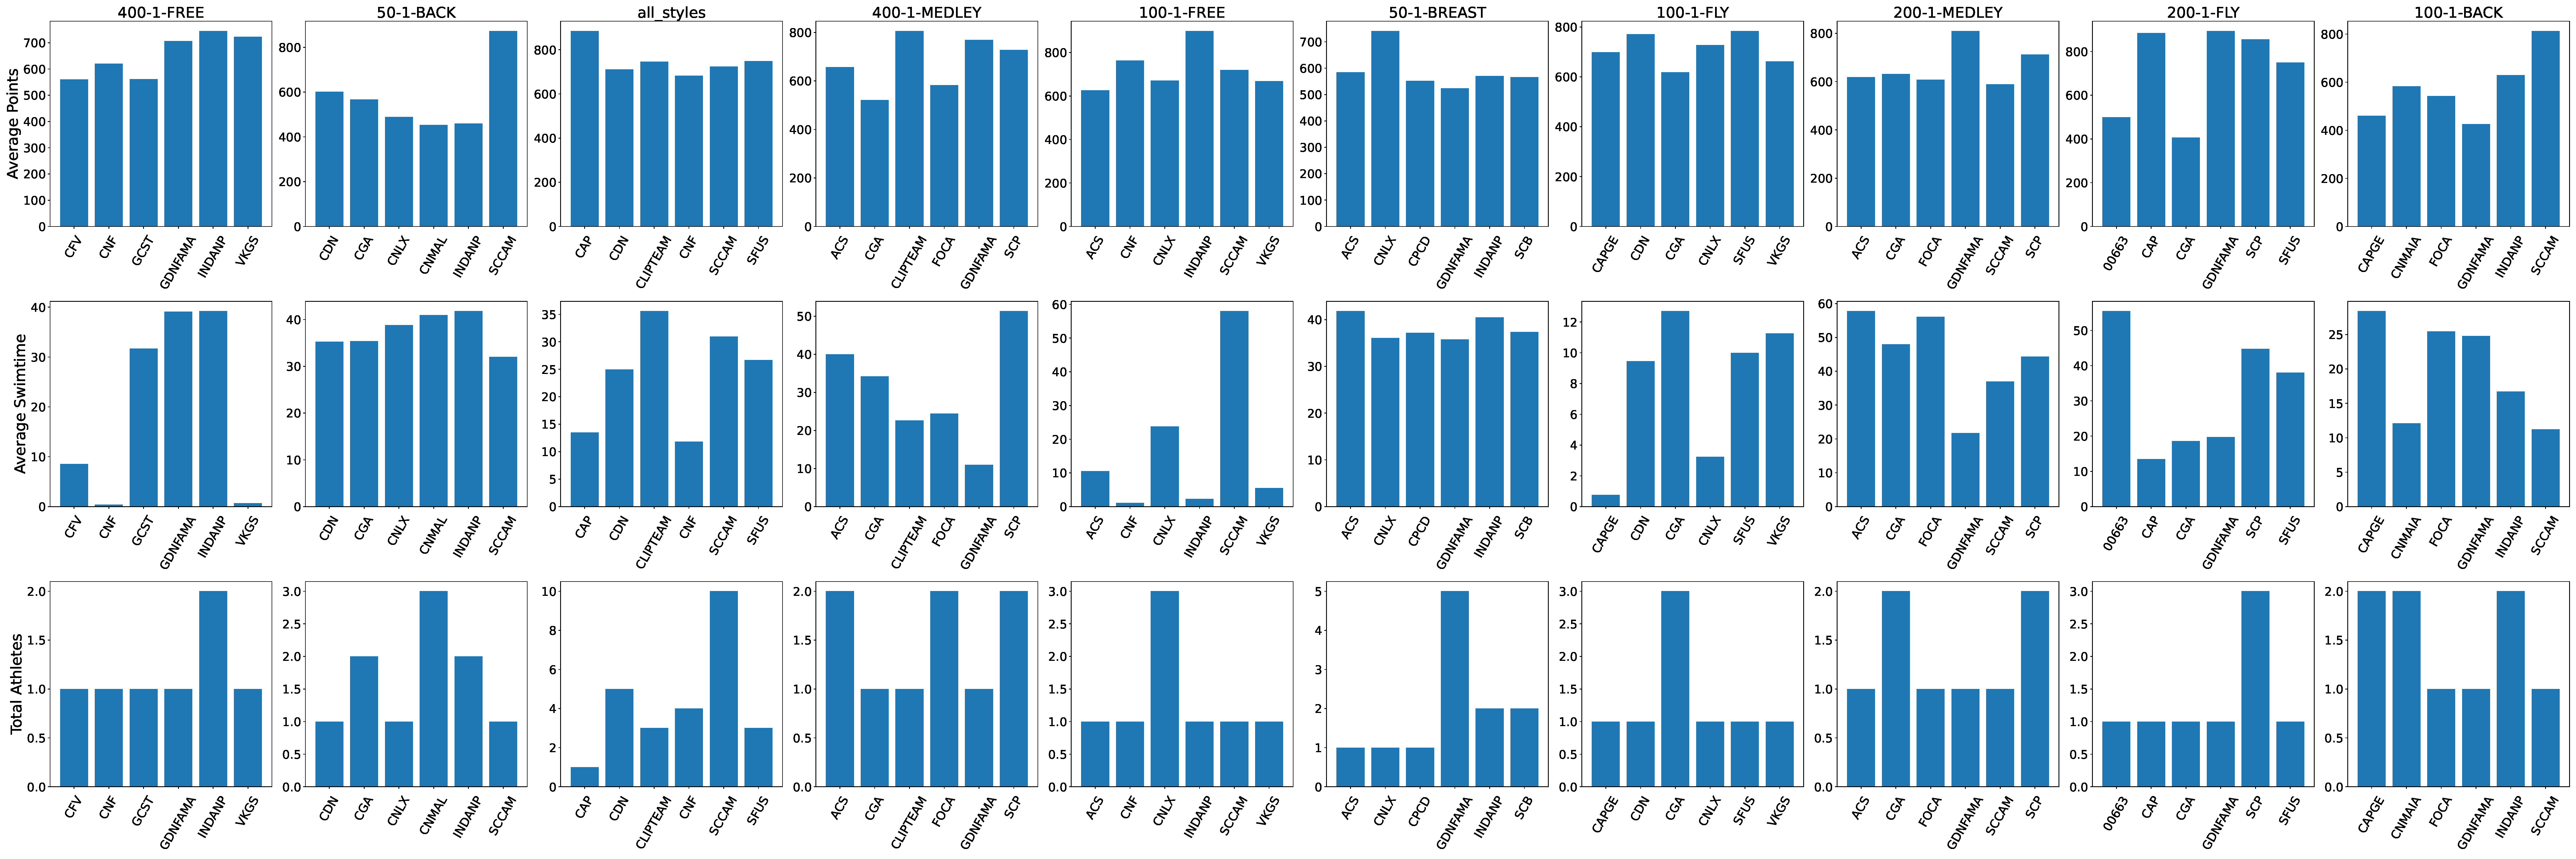
\includegraphics[width=\textwidth]{img/stats_clubs_swim.pdf}
    \caption{Top 5 teams per swim style for a given statistic.}
    \label{fig:clubs_fact2}
\end{figure}

\subsection{Athlete Facts Statistics}

\begin{minted}{sql}
SELECT
    CASE GROUPING(a.firstname)
        WHEN 1 THEN 'all_players'
        ELSE a.firstname
    END AS "Athletes",
    CASE GROUPING(af.meetid)
        WHEN 1 THEN 'all_meets'
        ELSE af.meetid
    END AS "Tournament",
    ROUND(AVG(average_points), 2) AS "Average Points",
    ROUND(AVG(average_distance), 2) AS "Average Distance",
    ROUND(AVG(average_swimtime), 2) AS "Average Swimtime"
FROM (
    SELECT
        athleteid,
        CAST(meetid as VARCHAR(255)),
        average_points,
        average_distance,
        average_swimtime
    FROM annp_final.athlete_defacto) af
JOIN annp_final.athlete a ON a.athleteid = af.athleteid
GROUP BY CUBE (a.firstname, af.meetid)
ORDER BY "Average Points" DESC
LIMIT 50;
\end{minted}


\begin{figure}[H]
    \centering
    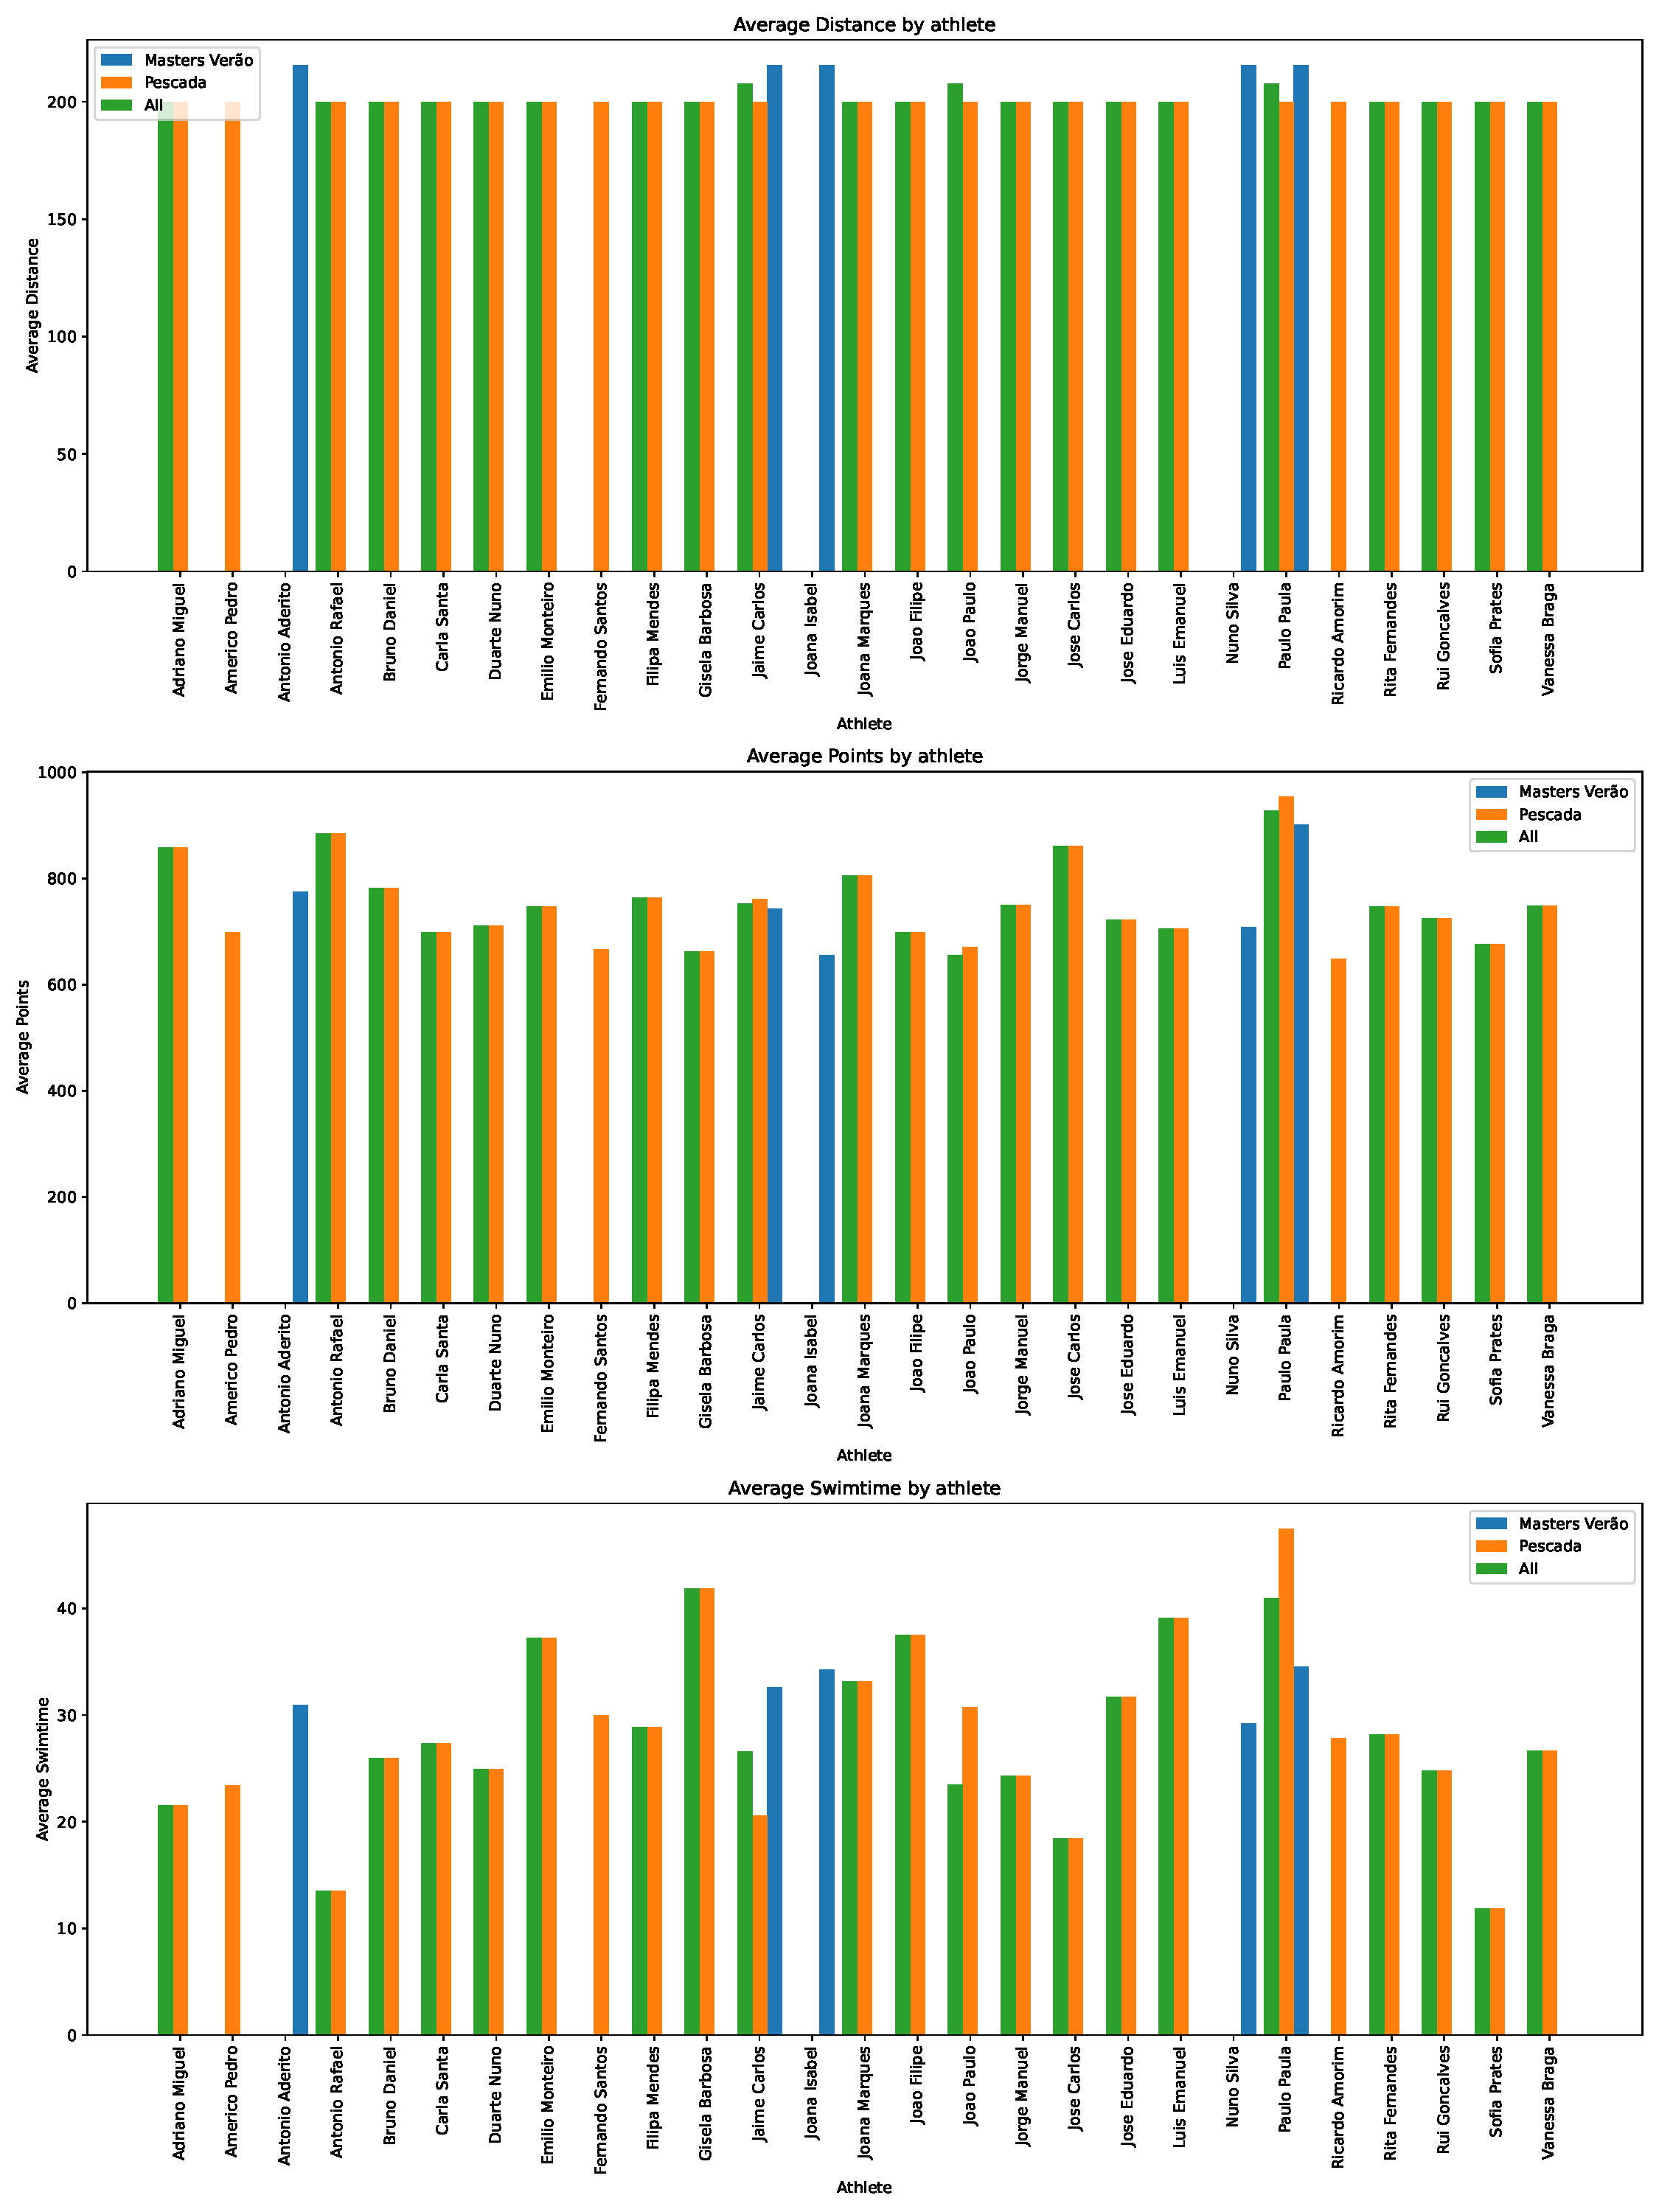
\includegraphics[width=\textwidth]{img/athletefact.pdf}
    \caption{Statistics from fact Club table.}
    \label{fig:athlete_fact}
\end{figure}

\pagebreak

\section{Conclusions \& Future Work} \label{sec:conclusion}

In this practical assignment, \textcolor{red}{COMPLETAR COM TEXTO} that allowed us to have a better insight into the data.

As future work, it would be important to include information about other tournaments in the database.
To do this, we would have to pre-process the data to ensure it conforms to the database schema.

\end{document}